\documentclass{beamer}

% Setup appearance:

\usetheme{Darmstadt}
\usefonttheme[onlylarge]{structurebold}
\setbeamerfont*{frametitle}{size=\normalsize,series=\bfseries}
\setbeamertemplate{navigation symbols}{}


% Standard packages

\usepackage[brazil]{babel}
\usepackage[latin1]{inputenc}
\usepackage{times}
\usepackage[T1]{fontenc}
%\usepackage[table]{xcolor}
 
% Setup TikZ

\usepackage{tikz}
\usetikzlibrary{arrows}
\tikzstyle{block}=[draw opacity=0.7,line width=1.4cm]

%diretório das figuras
\graphicspath{../article}

\title[Extreme Chock]{%
Nanograms%
}

\author[Souza,Medeiros,Santos,Ara�jo]{
     Danilo~Souza\and
     Hugo~Santos\and
     Iago~Medeiros\and
     Welton~Ara�jo
     }


\institute[Bel�m]{
  \inst{1}%
  Universidade Federal do Par�
  }
\date[Bel�m 2012]{
  14 de Maio de 2013
  }



\begin{document}

\begin{frame}
  \titlepage
\end{frame}


\section{Introdu��o}
\begin{frame}{Introdu��o}
  \begin{itemize}
    \item	PIC 16F877A
    \item	Sentido e tipo de passo de um motor
  \end{itemize}
    \begin{figure}[ht]
      \centering
      \includegraphics[width=5.0cm]{pic16f877a.jpg} \quad
      %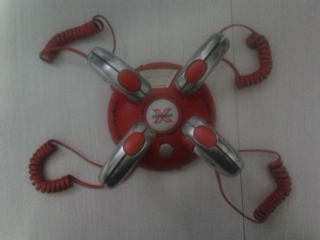
\includegraphics[width=5.0cm]{./article/dispositivo1.png}
  \end{figure}
\end{frame}

\section{Descri��o do projeto}
  \begin{frame}{Descri�ao do projeto}
	\begin{itemize}
	  \item 	1 bot�o para alternar entre sentido hor�rio e anti-hor�rio
	  \item		1 bot�o para alternar entre os tipos de passo simples 1, simples 2 e meio passo
	  \item		rotacionar o motor de passo de acordo com sentido e tipo de passo selecionado
	\end{itemize}
  \end{frame}
   
\section{Fluxograma}
  \begin{frame}{Fluxograma}
    \begin{figure}[ht]
	 \centering
	 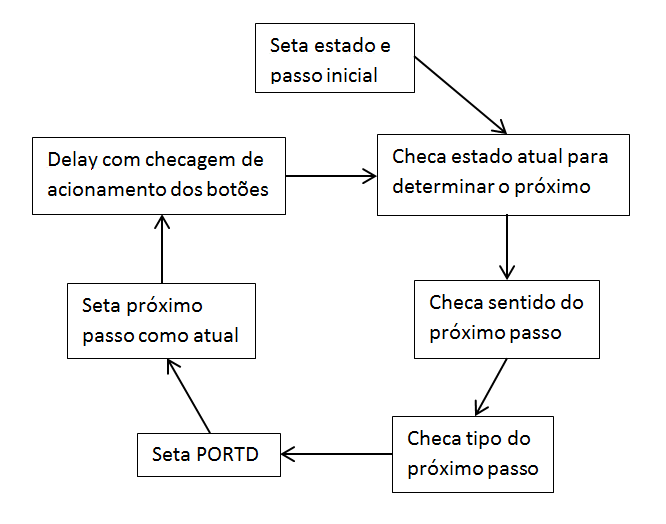
\includegraphics[width=9.0cm]{./article/fluxograma.png}
    \end{figure}      
  \end{frame}

\section{Rotinas}
  \begin{frame}{CHECK\_CUR\_STATE}
    \begin{figure}[ht]
	 \centering
	 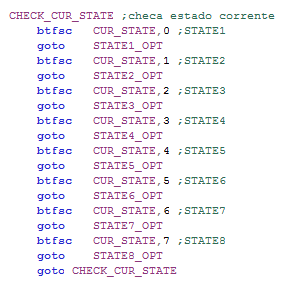
\includegraphics[width=7.0cm]{./check_cur_state.png}
    \end{figure}         
  \end{frame}
  \begin{frame}{STATE1\_OPT}
    \begin{figure}[ht]
	 \centering
	 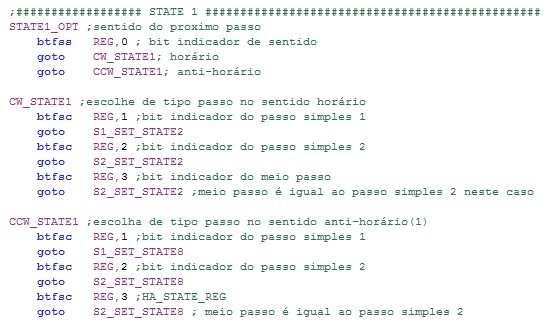
\includegraphics[width=11.0cm]{./state1_opt.png}
    \end{figure}         
  \end{frame}
  \begin{frame}{S1\_SET\_STATE1 E S2\_SET\_STATE1}
    \begin{figure}[ht]
	 \centering
	 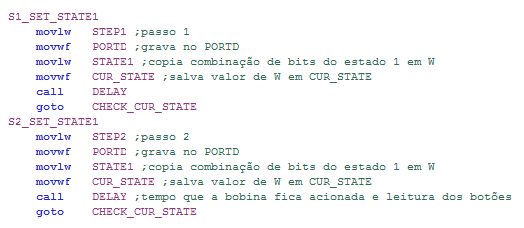
\includegraphics[width=11.0cm]{./set_state1.png}
    \end{figure}         
  \end{frame}
  

\section{Implementa��o no Proteus}
  \begin{frame}{Implementa�ao no Proteus}
	\begin{itemize}
	  \item 	2 pinos de entra no PORTD
	  \item		4 pinos de sa�da no PORTD
	  \item		2 bot�es
	  \item		1 motor de passo de 4 bobinas
	  \item		Inicia no sentido hor�rio
	  \item		Inicia com o passo simples 1
	  \item		Resposta r�pida
	  \end{itemize}
  \end{frame}

\end{document}
